\chapter{Fundamento te\'orico}

	En el tercer cap\'itulo se presentan las t\'ecnicas y herramientas utilizadas para adoptar una buena orientaci\'on que permita sustentar el desarrollo del Sistema Integral de indicadores mostrando una investigaci\'on detallada con todo lo necesario para entender cada fase del mismo.

	\section{Indicador}
		El primer concepto que nos debe quedar claro es saber que es un indicador, un indicador es un dato que nos ayuda a medir de manera objetiva la evoluci\'on de un sistema de gesti\'on, por consiguiente un sistema de indicadores son datos que nos brindan informaci\'on cualitativa o cuantitativa, que permiten seguir el desarrollo de un proceso y su evaluaci\'on.

	\section{Sistema de gest\'ion}
		Es una herramienta que permite a una organizaci\'on planear, ejecutar y controlar las actividades realizadas en esta, aquellas que sean necesarias para el buen desarrollo de su misi\'on. El objetivo de los sistemas es aportar a la instituci\'on  un camino correcto para lograr el cumplimiento de las metas establecidas. \\
	
	Todo sistema de medici\'on debe satisfacer los siguientes objetivos:

	\begin{itemize}
		\item Comunicar la estrategia.
		\item Comunicar las metas.
		\item Identificar problemas y oportunidades.
		\item Diagnosticar problemas.
		\item Entender procesos.
		\item Definir responsabilidades
		\item Mejorar el control de la instituci\'on.
		\item Identificar iniciativas y acciones necesarias.
		\item Medir comportamientos.
		\item Facilitar la delegaci\'on en las personas.
		\item Integrar la compensaci\'on con la actuaci\'on. 
	\end{itemize}

	El Sistema Integral de Indicadores es un sistema de gesti\'on que organiza indicadores, permitiendo mediante su implementaci\'on obtener m\'ultiples beneficios a la comunidad del Instituto Tecnol\'ogico de Tl\'ahuac los cuales son:
	\begin{itemize}
		\item Mejorar\'a la imagen ante los alumnos que deseen ingresar a dicha instituci\'on.
		\item Se lograra brindar un servicio caracterizado por la tolerancia y la responsabilidad.
		\item Permitir\'a contar con informaci\'on \'util para la mejora continua de procesos.
		\item Disminuir\'a las demoras en la realizaci\'on de tr\'amites internos.
		\item Se realizar\'a una gesti\'on enfocada al beneficio del alumno.
		\item Se Lograr\'a el compromiso de los directivos con los objetivos organizacionales.
		\item Permitir\'a conocer la informaci\'on de los avances en cuanto a la evaluaci\'on de procesos para poder tomar decisiones  estrat\'egicas y permitir alcanzar los objetivos.
	\end{itemize}

	Con dicho Sistema se pretende abarcar cada uno de los departamentos estrat\'egicos que sustentan al Instituto Tecnol\'ogico de Tl\'ahuac permitiendo a los directivos tener a su alcance los datos de los indicadores en cada uno de ellos, buscando una vinculaci\'on entre estos para obtener estad\'isticas correctas y precisas. Los departamentos abordados se muestran en la tabla \ref{tabDeptos}.

\begin{table}[h]
\centering
\caption{Tabla de departamentos organizadas por subdirecciones}
\label{tabDeptos}
\begin{tabular}{@{}cc@{}}
\toprule
\multirow{8}{*}{SUBDIRECCION ACAD\'EMICA}                                                                                   & CIENCIAS B\'ASICAS                                                                      \\ \cmidrule(l){2-2} 
& \multicolumn{1}{c}{CIENCIAS DE LA TIERRA}                                            \\ \cmidrule(l){2-2} 
& \multicolumn{1}{c}{ELECTRICA Y ELECTRONICA}                                          \\ \cmidrule(l){2-2} 
& \multicolumn{1}{c}{SISTEMAS Y COMPUTACION}                                           \\ \cmidrule(l){2-2} 
& \multicolumn{1}{c}{CIENCIAS ECON\'OMICO-ADMINISTRATIVAS}                               \\ \cmidrule(l){2-2} 
& \multicolumn{1}{c}{METAL-MEC\'ANICA}                                                   \\ \cmidrule(l){2-2} 
& \multicolumn{1}{c}{DESARROLLO ACAD\'EMICO}                                             \\ \cmidrule(l){2-2} 
& \multicolumn{1}{c}{DIVISI\'ON DE ESTUDIOS PROFESIONALES}                               \\ \midrule
\multicolumn{1}{c}{\multirow{5}{*}{SUBDIRECCI\'ON ADMINISTRATIVA}}                                                        & \multicolumn{1}{c}{RECURSOS HUMANOS}                                                 \\ \cmidrule(l){2-2} 
\multicolumn{1}{c}{}                                                                                                    & \multicolumn{1}{c}{RECURSOS FINANCIEROS}                                             \\ \cmidrule(l){2-2} 
\multicolumn{1}{c}{}                                                                                                    & \multicolumn{1}{c}{RECURSOS MATERIALES Y DE SERVICIOS}                               \\ \cmidrule(l){2-2} 
\multicolumn{1}{c}{}                                                                                                    & \multicolumn{1}{c}{CENTRO DE COMPUTO}                                                \\ \cmidrule(l){2-2} 
\multicolumn{1}{c}{}                                                                                                    & \multicolumn{1}{c}{MANTENIMIENTO Y EQUIPO}                                           \\ \midrule
\multicolumn{1}{c}{\multirow{6}{*}{\begin{tabular}[c]{@{}c@{}}SUBDIRECCI\'ON DE PLANEACI\'ON\\ Y VINCULACI\'ON\end{tabular}}} & \multicolumn{1}{c}{GESTI\'ON TECNOL\'OGICA Y VINCULACI\'ON}                                \\ \cmidrule(l){2-2} 
\multicolumn{1}{c}{}                                                                                                    & \multicolumn{1}{c}{COMUNICACI\'ON Y DIFUSI\'ON}                                          \\ \cmidrule(l){2-2} 
\multicolumn{1}{c}{}                                                                                                    & \multicolumn{1}{c}{ACTIVIDADES EXTRAESCOLARES}                                       \\ \cmidrule(l){2-2} 
\multicolumn{1}{c}{}                                                                                                    & \multicolumn{1}{c}{SERVICIOS ESCOLARES}                                              \\ \cmidrule(l){2-2} 
\multicolumn{1}{c}{}                                                                                                    & \multicolumn{1}{c}{CENTRO DE INFORMACI\'ON}                                            \\ \cmidrule(l){2-2} 
\multicolumn{1}{c}{}                                                                                                    & \begin{tabular}[c]{@{}c@{}}PLANEACI\'ON, PROGRAMACI\'ON \\ Y PRESUPUESTACI\'ON\end{tabular} \\ \bottomrule
\end{tabular}
\end{table}

Los departamentos antes mencionados se encuentran detallados en el sitio oficial del Instituto Tecnol\'ogico de Tl\'ahuac en la seccion de departamentos.\\

Para el desarrollo del Sistema Integral de Indicadores se realiz\'o una investigaci\'on acerca de las tecnolog\'ias que se utilizar\'ian. Estas se encuentran clasificadas en dos partes importantes en el desarrollo web, la parte del cliente y la parte del servidor.\\

Las tecnolog\'ias que se encuentran en la parte del cliente son todas aquellas que son ejecutadas por el navegador web como son Javascript, HTML y CSS.\\

Las tecnolog\'ias del lado del servidor son todas aquellas en las cuales su ejecuci\'on se encuentra del lado del servidor como son C\#, VB, Java, Python y PHP. Estos lenguajes tienen la capacidad de comunicarse directamente con la base de datos, y con esto realizar los procesos necesarios para formar el resultado solicitado por el cliente.\\ 	

Dentro de los lenguajes de servidor se encuentran los lenguajes de consulta de base de datos, los cuales como su nombre lo dice sirven para manipular la informaci\'on de una base de datos. El lenguaje de manipulaci\'on de datos que se utiliza en los diferentes motores de base de datos es SQL.\\ \\
A continuaci\'on se definir\'an las tecnolog\'ias del cliente utilizadas para el desarrollo del sistema.
\section{Arquitectura Cliente-Servidor}

Se puede definir la computacion cliente servidor  como una arquitectura  distribuida que permite obtener acceso a informacion de manera transparente para el usuario final aun en entornos multiplataforma.\\

La arquitectura cliente servidor es el resultado de la integracion de dos culturas, por un lado la del Mainframe que aporta la capacidad de almacenamiento, integridad y acceso a la informacion, y por otro lado la del computador, la cual aporta la facilidad de uso a bajo costo ademas, provee de una presentacion atractiva y una gran variedad en productos y aplicaciones.\\

El funcionamiento de la arquitectura cliente-servidor es la siguiente:

\begin{itemize}
	\item Solicitud de informaci�n del cliente al servidor.
	\item El servidor recibe la petici�n del cliente.
	\item El servidor procesa la solicitud.
	\item El servidor regresa el resultado con la informaci�n solicitada.
	\item El cliente recibe la informaci�n y la procesa.
\end{itemize}

La arquitectura cliente servidor est� basado en la idea del servicio, en el que el cliente es un proceso consumidor de servicios y el servidor es un proceso proveedor de servicios, esta relaci�n est� establecida en funci�n del intercambio de mensajes que es el �nico elemento de acoplamiento entre ambos.\\

Las partes fundamentales de la arquitectura cliente servidor son las siguientes:

\begin{itemize}
	\item \textbf{Proceso en el cliente:} Es el que inicia el dialogo mediante una petici�n.
	\item \textbf{Proceso en el servidor:} Es quien se encuentra en espera de que lleguen peticiones de servicio y da respuesta a las mismas.
	\item \textbf{Middleware:} Es el medio por el cual se transmite informaci�n entre cliente y servidor, permitiendo el env�o y recepci�n de mensajes.
\end{itemize}

En la figura X se muestra el diagrama que ilustra lo anterior.


	\begin{figure}[htb]
        \centering
        \includegraphics[width=14cm, height=9cm]{figuras/clienteservidor}
        \caption{Diagrama de modelo cliente-servidor.}
        \label{fig_clienteservidor}
    \end{figure}



\section{Lenguajes en cliente (Frontend)}
\subsection{HTML Y HTML 5}

Defini\'endolo de forma sencilla, \textsl{"HTML es lo que se utiliza para crear todas las p\'aginas web de Internet"}. M\'as concretamente, HTML es el lenguaje con el que se \textsl{"escriben"} la mayor\'ia de p\'aginas web.\\

Los dise\~nadores utilizan el lenguaje HTML para crear sus p\'aginas web, los programas que utilizan los dise\~nadores generan p\'aginas escritas en HTML y los navegadores que utilizamos los usuarios muestran las p\'aginas web despu\'es de leer su contenido HTML.\\

Aunque HTML es un lenguaje que utilizan los ordenadores y los programas de dise\~no, es muy f\'acil de aprender y escribir por parte de las personas.\\

El lenguaje HTML es un est\'andar reconocido en todo el mundo y cuyas normas define un organismo sin \'animo de lucro llamado World Wide Web Consortium, m\'as conocido como W3C. Como se trata de un est\'andar reconocido por todas las empresas relacionadas con el mundo de Internet, una misma p\'agina HTML se visualiza de forma muy similar en cualquier navegador de cualquier sistema operativo.\\

El propio W3C define el lenguaje HTML como \textsl{"un lenguaje reconocido universalmente y que permite publicar informaci\'on de forma global"}. Desde su creaci\'on, el lenguaje HTML ha pasado de ser un lenguaje utilizado exclusivamente para crear documentos electr\'onicos a ser un lenguaje que se utiliza en muchas aplicaciones electr\'onicas como buscadores, tiendas online y banca electr\'onica.\\

El origen de HTML se remonta al a\~no de 1980, cuando el f\'isico Tim Berners-Lee, trabajador del CERN propuso un nuevo sistema de hipertexto para compartir documentos.\\

Los sistemas de hipertexto hab\'ian sido desarrollados a\~nos antes. En el \'ambito de la inform\'atica el hipertexto permit\'ia que los usuarios accedieran a la informaci\'on relacionada con los documentos electr\'onicos que estaba visualizando. De cierta manera, los primitivos sistemas de hipertexto podr\'ian asimilarse a los enlaces de las p\'aginas web actuales.\\

Con el tiempo este sistema de hipertexto fue evolucionando convirti\'endose en el lenguaje de marcado m\'as utilizado en la actualidad, siendo su \'ultima versi\'on la conocida HTML5.\\

HTML5 establece una serie de nuevos elementos y atributos que reflejan el uso t\'ipico de los sitios web modernos, permitiendo concentrar b\'asicamente tres caracter\'isticas:

\begin{itemize}
	\item Estructura.
	\item Estilo.
	\item Funcionalidad.
\end{itemize}

Aunque oficialmente no fue declarado, HTML5 es considerado como la combinaci\'on de HTML, CSS y Javascript ya que estas tecnolog\'ias son altamente dependientes y act\'uan como una sola unidad organizada bajo  la especificaci\'on de HTML5. HTML est\'a a cargo de la estructura, CSS presenta esta estructura y Javascript se encarga de darle funcionalidad.

\subsection{CSS}

Como ya se mencion\'o anteriormente el conjunto de tecnolog\'ias que trabajan en conjunto con HTML para formar HTML5 no solamente incluye los nuevos elementos que permiten que la definici\'on de la estructura de un sistema se mas f\'acil, si no tambi\'en es de vital importancia hablar de la parte que permite darle una buena presentaci\'on.\\

Oficialmente CSS no tiene nada que ver con HTML5 ya que es un complemento desarrollado para superar las limitaciones y reducir la complejidad de HTML. En un principio HTML prove\'ia de atributos que permit\'ian definir estilos esenciales para cada elemento, pero a medida que el lenguaje evoluciono, la escritura de c\'odigos se volvi\'o compleja  y no pudo satisfacer las necesidades demandadas por los dise\~nadores, en consecuencia, CSS pronto fue adoptado gracias a que este permite separar la estructura de la presentaci\'on. Desde entonces CSS se ha convertido en uno de los lenguajes m\'as importantes de la actualidad enfocado en las necesidades de los dise\~nadores.\\

En la versi\'on 3 de CSS es considerado en el desarrollo de HTML5 , debido a esto la integraci\'on entre ambos lenguajes es vital para el desarrollo web  y es la raz\'on por la que cada que se habla de HTML5 tambi\'en se hace referencia a CSS3 aunque oficialmente se trate de dos tecnolog\'ias completamente separadas.
En estos momentos las nuevas caracter\'isticas que se incorporan a CSS3 se han ido incorporando a los navegadores web al igual que las caracter\'isticas de HTML5.

\subsection{Javascript}

Javascript es un lenguaje interpretado usado para m\'ultiples prop\'ositos pero solo considerado como un complemento hasta ahora. Una de las innovaciones que ayud\'o a cambiar el modo en que vemos Javascript fue el desarrollo de nuevos motores de interpretaci\'on, creados para acelerar el procesamiento de c\'odigo. La clave de los motores m\'as exitosos fue transformar el c\'odigo Javascript en c\'odigo m\'aquina para lograr velocidades de ejecuci\'on similares a aquellas encontradas en aplicaciones de escritorio. Esta mejorada capacidad permiti\'o superar viejas limitaciones de rendimiento y confirmar el lenguaje Javascript como la mejor opci\'on para la web.\\

Para aprovechar esta prometedora plataforma de trabajo ofrecida por los nuevos navegadores, Javascript fue expandido en relaci\'on con portabilidad e integraci\'on.Ala vez, interfaces de programaci\'on de aplicaciones (APIs) fueron incorporadas por defecto en cada navegador para asistir al lenguaje en funciones elementales. Estas nuevas APIs (como Web Storage, Canvas, y otras) son interfaces para librer\'ias incluidas en navegadores. La idea es hacer disponible poderosas funciones a trav\'es de t\'ecnicas de programaci\'on sencillas y est\'andares, expandiendo el alcance del lenguaje y facilitando la creaci\'on de programas \'utiles para la web.\\


Despues de hablar de las tecnolog\'ias del lado del cliente, a continuacion hablaremos de las que se ejecutan en el servidor.

\section{Lenguajes en servidor (Backend)}
\subsection{C\#}

C\# es el nuevo lenguaje de prop\'osito general dise\~nado por Scott Wiltamuth y Anders Hejlsberg, este \'ultimo tambi\'en es conocido por dise\~nar el lenguaje Turbo Pascal y la herramienta RAD Delphi.\\

Aunque es posible escribir c\'odigo para la plataforma .NET en distintos lenguajes, C\# es el \'unico dise\~nado espec\'ificamente para ser utilizado en ella, por lo que programarla usando C\# es mucho m\'as sencillo e intuitivo que hacerlo con cualquiera de los otros lenguajes ya que C\# carece de elementos heredados innecesarios en .NET. Por esta raz\'on, se suele decir que C\# es el lenguaje nativo de .NET.\\

En resumen, C\# es un lenguaje de programaci\'on que toma las mejores caracter\'isticas de lenguajes preexistentes como Visual Basic, Java o C++ y las combina en uno solo. El hecho de ser relativamente reciente no implica que sea inmaduro, pues Microsoft ha escrito la mayor parte de la BCL us\'andolo, por lo que su compilador es el m\'as depurado y optimizado de los incluidos en el .NET Framework SDK.\\

Las caracter\'isticas principales de C\# son las siguientes:
\begin{itemize}
	\item \textbf{Sencillez:} C\# elimina muchos elementos que otros lenguajes incluyen y que son innecesarios en .NET. Por ejemplo: 
		\begin{itemize}
			\item El c\'odigo escrito en C\# es auto contenido, lo que significa que no necesita de ficheros adicionales al propio fuente tales como ficheros de cabecera o ficheros IDL.
			\item El tama\~no de los tipos de datos b\'asicos es fijo e independiente del compilador, sistema operativo o m\'aquina para quienes se compile (no como en C++), lo que facilita la portabilidad del c\'odigo.
			\item No se incluyen elementos poco \'utiles de lenguajes como C++ tales como macros, herencia m\'ultiple o la necesidad de un operador diferente del punto (.) acceder a miembros de espacios de nombres (::) 
		\end{itemize}
		\item \textbf{Modernidad: } C\# incorpora en el propio lenguaje elementos que a lo largo de los a\~nos ha ido demostr\'andose son muy \'utiles para el desarrollo de aplicaciones y que en otros lenguajes como Java o C++ hay que simular, como un tipo b\'asico decimal que permita realizar operaciones de alta precisi\'on con reales de 128 bits, la inclusi\'on de una instrucci\'on foreach que permita recorrer colecciones con facilidad y es ampliable a tipos definidos por el usuario, la inclusi\'on de un tipo b\'asico string para representar cadenas o la distinci\'on de un tipo bool espec\'ifico para representar valores l\'ogicos. 
		
		\item \textbf{Orientaci\'on a objetos: }Como todo lenguaje de programaci\'on de prop\'osito general actual, C\# es un lenguaje orientado a objetos, aunque eso es m\'as bien una caracter\'istica del CTS que de C\#. Una diferencia de este enfoque orientado a objetos respecto al de otros lenguajes como C++ es que el de C\# es m\'as puro en tanto que no admiten ni funciones ni variables globales sino que todo el c\'odigo y datos han de definirse dentro de definiciones de tipos de datos, lo que reduce problemas por conflictos de nombres y facilita la legibilidad del c\'odigo.\\

		C\# soporta todas las caracter\'isticas propias del paradigma de programaci\'on orientada a objetos: encapsulaci\'on, herencia y polimorfismo.\\

		En lo referente a la encapsulaci\'on es importante se\~nalar que aparte de los t\'ipicos modificadores public, private y protected, C\# a\~nade un cuarto modificador llamado internal, que puede combinarse con protected e indica que al elemento a cuya definici\'on precede s\'olo puede accederse desde su mismo ensamblado.\\

		Respecto a la herencia -a diferencia de C++ y al igual que Java- C\# s\'olo admite herencia simple de clases ya que la m\'ultiple provoca m\'as quebraderos de cabeza que facilidades y en la mayor\'ia de los casos su utilidad puede ser simulada con facilidad mediante herencia m\'ultiple de interfaces. De todos modos, esto vuelve a ser m\'as bien una caracter\'istica propia del CTS que de C\#.\\

		Por otro lado y a diferencia de Java, en C\# se ha optado por hacer que todos los m\'etodos sean por defecto sellados y que los redefinibles hayan de marcarse con el modificador virtual (como en C++), lo que permite evitar errores derivados de redefiniciones accidentales. Adem\'as, un efecto secundario de esto es que las llamadas a los m\'etodos ser\'an m\'as eficientes por defecto al no tenerse que buscar en la tabla de funciones virtuales la implementaci\'on de los mismos a la que se ha de llamar. Otro efecto secundario es que permite que las llamadas a los m\'etodos El lenguaje de programaci\'on C\# Tema 2: Introducci\'on a C\# Jos\'e Antonio Gonz\'alez Seco P\'agina 23 virtuales se puedan hacer m\'as eficientemente al contribuir a que el tama\~no de dicha tabla se reduzca. 

		\item \textbf{Orientaci\'on a componentes: } La propia sintaxis de C\# incluye elementos propios del dise\~no de componentes que otros lenguajes tienen que simular mediante construcciones m\'as o menos complejas. Es decir, la sintaxis de C\# permite definir c\'omodamente propiedades (similares a campos de acceso controlado), eventos (asociaci\'on controlada de funciones de respuesta a notificaciones) o atributos (informaci\'on sobre un tipo o sus miembros).

		\item \textbf{Gesti\'on autom\'atica de memoria: } Como ya se coment\'o, todo lenguaje de .NET tiene a su disposici\'on el recolector de basura del CLR. Esto tiene el efecto en el lenguaje de que no es necesario incluir instrucciones de destrucci\'on de objetos. Sin embargo, dado que la destrucci\'on de los objetos a trav\'es del recolector de basura es indeterminista y s\'olo se realiza cuando \'este se active ya sea por falta de memoria, finalizaci\'on de la aplicaci\'on o solicitud expl\'icita en el fuente-, C\# tambi\'en proporciona un mecanismo de liberaci\'on de recursos determinista a trav\'es de la instrucci\'on using. 

		\item \textbf{Seguridad de tipos: } C\# incluye mecanismos que permiten asegurar que los accesos a tipos de datos siempre se realicen correctamente, lo que permite evita que se produzcan errores dif\'iciles de detectar por acceso a memoria no perteneciente a ning\'un objeto y es especialmente necesario en un entorno gestionado por un recolector de basura. Para ello se toman medidas del tipo: 
		\begin{itemize}
			\item S\'olo se admiten conversiones entre tipos compatibles. Esto es, entre un tipo y antecesores suyos, entre tipos para los que expl\'icitamente se haya definido un operador de conversi\'on, y entre un tipo y un tipo hijo suyo del que un objeto del primero almacenase una referencia del segundo (downcasting) Obviamente, lo \'ultimo s\'olo puede comprobarlo en tiempo de ejecuci\'on el CLR y no el compilador, por lo que en realidad el CLR y el compilador colaboran para asegurar la correcci\'on de las conversiones. 
			\item No se pueden usar variables no inicializadas. El compilador da a los campos un valor por defecto consistente en ponerlos a cero y controla mediante an\'alisis del flujo de control del fuente que no se lea ninguna variable local sin que se le haya asignado previamente alg\'un valor. 
			\item Se comprueba que todo acceso a los elementos de una tabla se realice con \'indices que se encuentren dentro del rango de la misma. 
			\item Se puede controlar la producci\'on de desbordamientos en operaciones aritm\'eticas, inform\'andose de ello con una excepci\'on cuando ocurra. Sin embargo, para conseguirse un mayor rendimiento en la aritm\'etica estas comprobaciones no se hacen por defecto al operar con variables sino s\'olo con constantes (se pueden detectar en tiempo de compilaci\'on).
			\item A diferencia de Java, C\# incluye delegados, que son similares a los punteros a funciones de C++ pero siguen un enfoque orientado a objetos, pueden almacenar referencias a varios m\'etodos simult\'aneamente, y se comprueba que los m\'etodos a los que apunten tengan par\'ametros y valor de retorno del tipo indicado al definirlos. 
			\item Pueden definirse m\'etodos que admitan un n\'umero indefinido de par\'ametros de un cierto tipo, y a diferencia lenguajes como C/C++, en C\# siempre se comprueba que los valores que se les pasen en cada llamada sean de los tipos apropiados. 
		\end{itemize}
	\item \textbf{Instrucciones seguras: } Para evitar errores muy comunes, en C\# se han impuesto una serie de restricciones en el uso de las instrucciones de control m\'as comunes. Por ejemplo, la guarda de toda condici\'on ha de ser una expresi\'on condicional y no aritm\'etica, con lo que se evitan errores por confusi\'on del operador de igualdad (==) con el de asignaci\'on (=); y todo caso de un switch ha de terminar en un break o goto que indique cu\'al es la siguiente acci\'on a realizar, lo que evita la ejecuci\'on accidental de casos y facilita su reordenaci\'on.

	\item \textbf{Sistema de tipos unificado: } A diferencia de C++, en C\# todos los tipos de datos que se definan siempre derivar\'an, aunque sea de manera impl\'icita, de una clase base com\'un llamada System.Object, por lo que dispondr\'an de todos los miembros definidos en \'esta clase (es decir, ser\'an "objetos").\\

	A diferencia de Java, en C\# esto tambi\'en es aplicable a los tipos de datos b\'asicos Adem\'as, para conseguir que ello no tenga una repercusi\'on negativa en su nivel de rendimiento, se ha incluido un mecanismo transparente de boxing y unboxing con el que se consigue que s\'olo sean tratados como objetos cuando la situaci\'on lo requiera, y mientras tanto puede aplic\'arseles optimizaciones espec\'ificas.\\

	El hecho de que todos los tipos del lenguaje deriven de una clase com\'un facilita enormemente el dise\~no de colecciones gen\'ericas que puedan almacenar objetos de cualquier tipo. 

	\item \textbf{Extensibilidad de tipos b\'asicos: }  C\# permite definir, a trav\'es de estructuras, tipos de datos para los que se apliquen las mismas optimizaciones que para los tipos de datos b\'asicos. Es decir, que se puedan almacenar directamente en pila (luego su creaci\'on, destrucci\'on y acceso ser\'an m\'as r\'apidos) y se asignen por valor y no por referencia. Para conseguir que lo \'ultimo no tenga efectos negativos al pasar estructuras como par\'ametros de m\'etodos, se da la posibilidad de pasar referencias a pila a trav\'es del modificador de par\'ametro ref. 

	\item \textbf{Extensibilidad de operadores: } Para facilitar la legibilidad del c\'odigo y conseguir que los nuevos tipos de datos b\'asicos que se definan a trav\'es de las estructuras est\'en al mismo nivel que los b\'asicos predefinidos en el lenguaje, al igual que C++ y a diferencia de Java, C\# permite redefinir el significado de la mayor\'ia de los operadores -incluidos los de conversi\'on, tanto para conversiones impl\'icitas como expl\'icitas- cuando se apliquen a diferentes tipos de objetos.\\

	Las redefiniciones de operadores se hacen de manera inteligente, de modo que a partir de una \'unica definici\'on de los operadores ++ y -- el compilador puede deducir autom\'aticamente como ejecutarlos de manera prefijas y postifja; y definiendo operadores simples (como +), el compilador deduce c\'omo aplicar su versi\'on de asignaci\'on compuesta (+=). Adem\'as, para asegurar la consistencia, el compilador vigila que los operadores con opuesto siempre se redefinan por parejas (por ejemplo, si se redefine ==, tambi\'en hay que redefinir !=).\\

	Tambi\'en se da la posibilidad, a trav\'es del concepto de indizador, de redefinir el significado del operador [] para los tipos de dato definidos por el usuario, con lo que se consigue que se pueda acceder al mismo como si fuese una tabla. Esto es muy \'util para trabajar con tipos que act\'uen como colecciones de objetos. 

	\item \textbf{Extensibilidad de modificadores: } C\# ofrece, a trav\'es del concepto de atributos, la posibilidad de a\~nadir a los metadatos del m\'odulo resultante de la compilaci\'on de cualquier fuente informaci\'on adicional a la generada por el compilador que luego podr\'a ser consultada en tiempo ejecuci\'on a trav\'es de la librer\'ia de reflexi\'on de .NET . Esto, que m\'as bien es una caracter\'istica propia de la plataforma .NET y no de C\#, puede usarse como un mecanismo para definir nuevos modificadores. 

	\item \textbf{Versionable: } C\# incluye una pol\'itica de versionado que permite crear nuevas versiones de tipos sin temor a que la introducci\'on de nuevos miembros provoquen errores dif\'iciles de detectar en tipos hijos previamente desarrollados y ya extendidos con miembros de igual nombre a los reci\'en introducidos.\\

	Si una clase introduce un nuevo m\'etodo cuyas redefiniciones deban seguir la regla de llamar a la versi\'on de su padre en alg\'un punto de su c\'odigo, dif\'icilmente seguir\'ian esta regla miembros de su misma signatura definidos en clases hijas previamente a la definici\'on del mismo en la clase padre; o si introduce un nuevo campo con el mismo nombre que alg\'un m\'etodo de una clase hija, la clase hija dejar\'a de funcionar. Para evitar que esto ocurra, en C\# se toman dos medidas: 
	\begin{itemize}
		\item Se obliga a que toda redefinici\'on deba incluir el modificador override, con lo que la versi\'on de la clase hija nunca ser\'ia considerada como una redefinici\'on de la versi\'on de miembro en la clase padre ya que no incluir\'ia override. Para evitar que por accidente un programador incluya este modificador, s\'olo se permite incluirlo en miembros que tengan la misma signatura que miembros marcados como redefinibles mediante el modificador virtual. As\'i adem\'as se evita el error tan frecuente en Java de creerse haber redefinido un miembro, pues si el miembro con override no existe en la clase padre se producir\'a un error de compilaci\'on. 

		\item Si no se considera redefinici\'on, entonces se considera que lo que se desea es ocultar el m\'etodo de la clase padre, de modo que para la clase hija sea como si nunca hubiese existido. El compilador avisar\'a de esta decisi\'on a trav\'es de un mensaje de aviso que puede suprimirse incluyendo el modificador new en la definici\'on del miembro en la clase hija para as\'i indicarle expl\'icitamente la intenci\'on de ocultaci\'on. 
	\end{itemize}

	\item \textbf{Eficiente: } En principio, en C\# todo el c\'odigo incluye numerosas restricciones para asegurar su seguridad y no permite el uso de punteros. Sin embargo, y a diferencia de Java, en C\# es posible saltarse dichas restricciones manipulando El lenguaje de programaci\'on C\# Tema 2: Introducci\'on a C\# Jos\'e Antonio Gonz\'alez Seco P\'agina 26 objetos a trav\'es de punteros. Para ello basta marcar regiones de c\'odigo como inseguras (modificador unsafe) y podr\'an usarse en ellas punteros de forma similar a c\'omo se hace en C++, lo que puede resultar vital para situaciones donde se necesite una eficiencia y velocidad procesamiento muy grandes. 

	\item \textbf{Compatible: } Para facilitar la migraci\'on de programadores, C\# no s\'olo mantiene una sintaxis muy similar a C, C++ o Java que permite incluir directamente en c\'odigo escrito en C\# fragmentos de c\'odigo escrito en estos lenguajes, sino que el CLR tambi\'en ofrece, a trav\'es de los llamados Platform Invocation Services (PInvoke), la posibilidad de acceder a c\'odigo nativo escrito como funciones sueltas no orientadas a objetos tales como las DLLs de la API Win32. N\'otese que la capacidad de usar punteros en c\'odigo inseguro permite que se pueda acceder con facilidad a este tipo de funciones, ya que \'estas muchas veces esperan recibir o devuelven punteros.\\

	Tambi\'en es posible acceder desde c\'odigo escrito en C\# a objetos COM. Para facilitar esto, el .NET Framework SDK incluye una herramientas llamadas tlbimp y regasm mediante las que es posible generar autom\'aticamente clases proxy que permitan, respectivamente, usar objetos COM desde .NET como si de objetos .NET se tratase y registrar objetos .NET para su uso desde COM.\\

	Finalmente, tambi\'en se da la posibilidad de usar controles ActiveX desde c\'odigo .NET y viceversa. Para lo primero se utiliza la utilidad aximp, mientras que para lo segundo se usa la ya mencionada regasm.
\end{itemize}


\subsection{Bootstrap}

Para comenzar a hablar de bootstrap es necesario citar algunas definiciones las cuales aclararan el panorama acerca de este.

	\subsection{Framework}

	El concepto framework se emplea en muchos \'ambitos del desarrollo de sistemas software, no solo en el \'ambito de aplicaciones Web. Podemos encontrar frameworks para el desarrollo de aplicaciones m\'edicas, de visi\'on por computador, para el desarrollo de juegos, y para cualquier \'ambito que pueda ocurr\'irsenos.\\

 	En general, con el t\'ermino framework, nos estamos refiriendo a una estructura software compuesta de componentes personalizables e intercambiables para el desarrollo de una aplicaci\'on. En otras palabras, un framework se puede considerar como una aplicaci\'on gen\'erica incompleta y configurable a la que podemos a\~nadirle las \'ultimas piezas para construir una aplicaci\'on concreta.
